\documentclass[tikz]{standalone}
\usepackage{tikz}
\usetikzlibrary{calc,positioning, shapes, petri, automata}
\tikzset{
    transV/.style={transition, fill=black,font=\footnotesize, minimum height = 12mm, minimum width = 1.5mm,inner sep = 0mm},
    transH/.style={transition, fill=black,font=\footnotesize, minimum width = 12mm, minimum height = 1.5mm,inner sep = 0mm},
    node distance=1.5
}
\usepackage{amsmath,amssymb,amsthm,mathrsfs,amsfonts}

\usepackage{csquotes}
\usepackage{booktabs}

\usepackage{graphicx}
\graphicspath{ {../img/} }

\newcommand{\LSset}[2]{\scriptsize $\begin{aligned}&\{#1\}_L\\&\{#2\}_S\end{aligned}$}


\begin{document}    
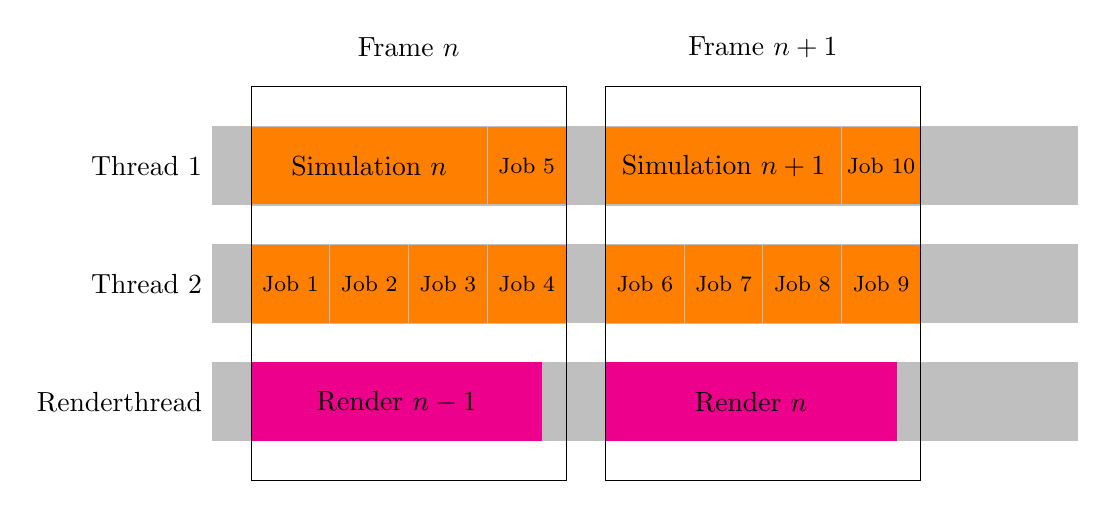
\begin{tikzpicture}
	\fill[lightgray]  (0,0) rectangle (11,1);
	\fill[lightgray] (0,-1.5) rectangle (11,-0.5);
	\fill[lightgray]  (0,1.5) rectangle (11,2.5);
	
	\node[anchor=east] at (0,2) {Thread 1};
	\node[anchor=east] at (0,0.5) {Thread 2};
	\node[anchor=east] at (0,-1) {Renderthread};
	
	
	\fill [orange,draw=lightgray] (0.5,1.5) rectangle node[black] {Simulation $n$} (3.5,2.5);
	\fill [orange,draw=lightgray] (3.5,1.5) rectangle node[black,font=\footnotesize] {Job 5} (4.5,2.5);
	\fill [orange,draw=lightgray] (0.5,0) rectangle node[black,font=\footnotesize] {Job 1} (1.5,1);
	\fill [orange,draw=lightgray] (1.5,0) rectangle node[black,font=\footnotesize] {Job 2} (2.5,1);
	\fill [orange,draw=lightgray] (2.5,0) rectangle node[black,font=\footnotesize] {Job 3} (3.5,1);
	\fill [orange,draw=lightgray] (3.5,0) rectangle node[black,font=\footnotesize] {Job 4} (4.5,1);

	\fill [orange,draw=lightgray] (5,1.5) rectangle node[black] {Simulation $n+1$} (8,2.5);
	\fill [orange,draw=lightgray] (5,0) rectangle node[black,font=\footnotesize] {Job 6} (6,1);
	\fill [orange,draw=lightgray] (6,0) rectangle node[black,font=\footnotesize] {Job 7} (7,1);
	\fill [orange,draw=lightgray] (7,0) rectangle node[black,font=\footnotesize] {Job 8} (8,1);
	\fill [orange,draw=lightgray] (8,0) rectangle node[black,font=\footnotesize] {Job 9} (9,1);
	\fill [orange,draw=lightgray] (8,1.5) rectangle node[black,font=\footnotesize] {Job 10} (9,2.5);

	\fill [magenta] (0.5,-0.5) rectangle node[black]{Render $n-1$} (4.2,-1.5);
	\fill [magenta] (5,-0.5) rectangle node[black]{Render $n$} (8.7,-1.5);
	
	\node at (2.5,3.5) {Frame $n$};
	\node at (7,3.5) {Frame $n+1$};
	
	\draw  (0.5,3) rectangle (4.5,-2);
	\draw  (5,3) rectangle (9,-2);
\end{tikzpicture}
\end{document}